\documentclass[12pt,draft]{article}
\usepackage[utf8]{inputenc}
\usepackage{geometry}
\usepackage{tabularray}
\usepackage{etoolbox}
\usepackage{graphicx}

\geometry{letterpaper, margin=1in}

\renewcommand{\familydefault}{\sfdefault}
\frenchspacing

\graphicspath{{./Graphics/Output/}}

\pagestyle{myheadings}
\markright{Orion Capsule Repair Manual}

\AddToHook{cmd/section/before}{\clearpage}

\def\overview{\subsubsection*{Overview}}
\def\instruc{\subsubsection*{Repair Instructions}}

\newcommand{\status}[1]{\fbox{\texttt{#1}}}

\newcommand{\maybedot}[2]{\ifstrequal{#1}{#2}{\textbullet}{}}
\newcommand{\hstable}[2]{
 \begin{tblr}{
  hlines, vlines,
  hline{2} = {2pt, solid},
  rows = {0.5cm, m}, columns = {0.5cm,c},
  cell{1}{1} = {r=1,c=3}{c}
 }
  #1 & & \\
  \maybedot{#2}{1} & \maybedot{#2}{2} & \maybedot{#2}{3} \\
  \maybedot{#2}{4} & \maybedot{#2}{5} & \maybedot{#2}{6}
 \end{tblr}
}

\begin{document}

\begin{titlepage}
 \thispagestyle{empty}
 \centering
 \rmfamily
 {\Huge\bfseries Orion Capsule Repair Manual\par}
 \vspace{1cm}
 {\Large Mission Control Guide}
 \vfill
\end{titlepage}

\section*{Introduction}

Although everything possible is done beforehand to limit the possibility of the spacecraft being damaged during a mission, it is still a scenario that both the crew of the spacecraft and Mission Control must be prepared for. This manual has been written to assist Mission Control in guiding the astronauts through the progress of diagnosing and fixing issues that may arise with the Orion capsule.

\subsection*{Time}

First and foremost, it is of the utmost importance that problems be fixed in a timely manner. In a situation in which a second can mean the difference between mission success and failure, diagnosing and fixing issues is a matter of extreme urgency. In short: time is of the essence! In an emergency situation, all astronauts will be relayed the remaining window to fix all issues with the spacecraft before the mission must be aborted. The crew and Mission Control must therefore communicate quickly and effectively. However, although members of the crew and Mission Control must act quickly, they must also act cautiously, as taking the wrong action could further jeopardize the mission!

\subsection*{System Modules}

Throughout the interior of the Orion capsule, several panels can be found. Each one interfaces with a different essential system in the spacecraft and can be used to detect and fix problems. Should any problems arise, it is imperative that the astronauts make an exhaustive search of the capsule interior for panels with an error status. All surfaces of the capsule should be thouroughly searched. Each panel has a title on the top indicating which system it is connected to and a status indicator on the top-right consisting of a two-character display that conveys information about the state of the connected system through the code it displays. Below the title and status indicator is the system interface, which contains elements allowing astronauts to interact with the system in order to repair it. If the system is repaired or progress is made, this may be deduced from the status code. Thus, it is important for the astronauts to relay the status code of a given panel and any changes thereto to Mission Control, so that they may identify any essential information carried by it using this manual.

\section*{Panel Usage}
\AddToHook{cmd/subsection/before}{\clearpage}

This section details the operation and functionality of each type of panel present in the interior of the Orion capsule. To diagnose and fix issues with a given panel, consult the corresponding subsection and follow the instructions given.

\subsection*{Propulsion System}

\overview

In order for the propulsion system to work properly, it is important to ensure that all of the electrical components involved are correctly connected. In the event of a propulsion system failure, the wires must be checked and reconnected so that the correct configuration is achieved for the launch sequence.

\instruc

\subsection*{Heat Shield}

\overview

To repair the heat shield, it is necessary to regonfigure the six-block control panel in order to provide full protection for the vehicle.

\instruc

The heat shield interface has two parts: a display at the top and six buttons arranged in a grid. Multiple rounds of reconfiguration may be necessary; if the heat shield has been damaged, the status indicator will display the number of rounds of reconfiguration necessary to fully repair it. The display will show a word. In order to perform the reconfiguration, read the button corresponding to the word in the table below.

\begin{center}
\begin{tblr}{
 rows = {m}, columns = {c}
}
\hstable{a}{4} & \hstable{b}{1} & \hstable{c}{3} & \hstable{d}{5} \\
\hstable{e}{0} & \hstable{f}{2} & \hstable{g}{3} & \hstable{h}{0} \\
\hstable{i}{1} & \hstable{j}{4} & \hstable{k}{5} & \hstable{l}{2}
\end{tblr}
\end{center}

Next, find the row in the table below corresponding to the word on the button read and press the button containing the first word that appears in the corresponding list, and you will move to the next round.

\begin{center}
\begin{tblr}{
 hlines, vlines,
 rows = {m}, colspec = {Q[c]Q[l]}
}
 a & f, h, j, l \\
 b & h, c, a, d \\
 c & b, g, a, e \\
 d & i, f, e, j \\
 e & d, l, h, k \\
 f & g, i, c, f \\
 g & l, j, f, a \\
 h & d, c, b, g \\
 i & j, a, i, b \\
 j & e, f, k, c \\
 k & f, d, k, h \\
 l & c, e, b, a
\end{tblr}
\end{center}

Once all rounds have been completed, the status indicator will show the code \status{BB} to signal that no more rounds of reconfiguration and the heat shield has returned to proper functionality.

\subsection*{Radiation Protection System}

\overview

Due to the extreme forces incurred by the spacecraft during flight, the radiation control filters may become misaligned. When this happens, it is necessary to realign them to ensure complete protection from radiation in the Van Allen Belt.

\instruc

On the control panel, a grid is displayed with four buttons below it, each with an arrow facing a different direction. There is also a Submit button below these. One square in the grid will be highlighted; this square represents the current orientation of the control filter. Use the panel status to determine the layout of the filter space according to the diagram below. The target position of the filter in each layout is marked with a dot. The lines between the spaces represent the movement contstraints of the filter; they can be treated as barriers that the filters path cannot cross.

\begin{center}
\begin{tblr}{
 rows = {m}, columns = {c},
 colsep = 4pt
}
 \status{AE} & \status{AE} & \status{AE}\\
 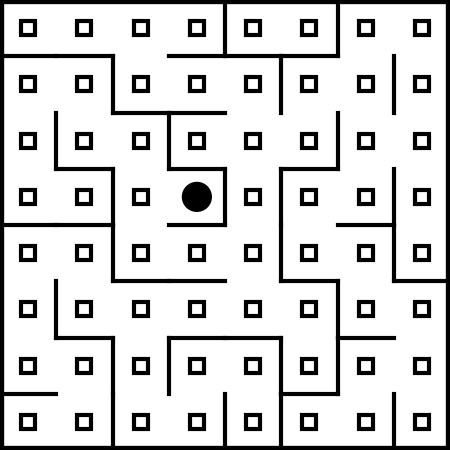
\includegraphics[width=2in]{AE} & 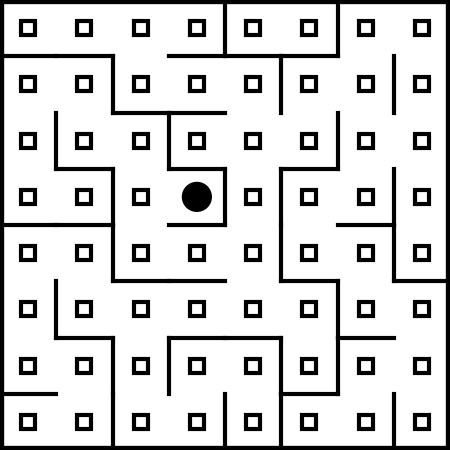
\includegraphics[width=2in]{AE} & 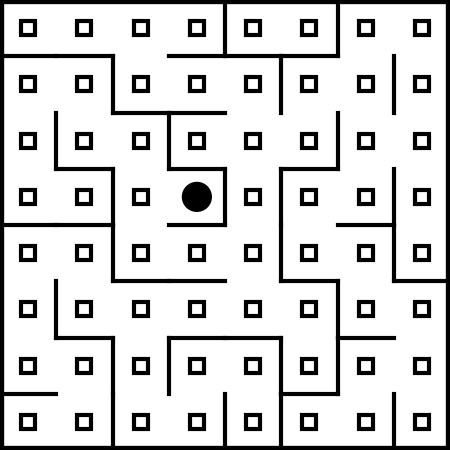
\includegraphics[width=2in]{AE}\\
 \status{AE} & \status{AE} & \status{AE}\\
 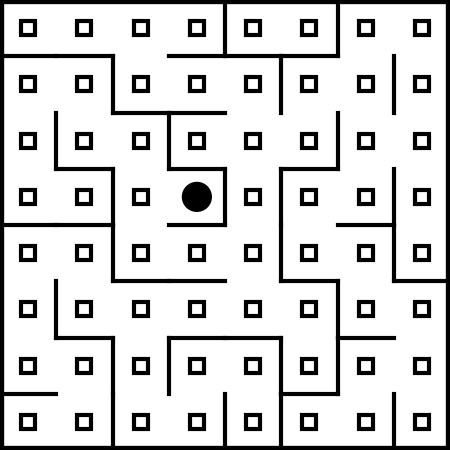
\includegraphics[width=2in]{AE} & 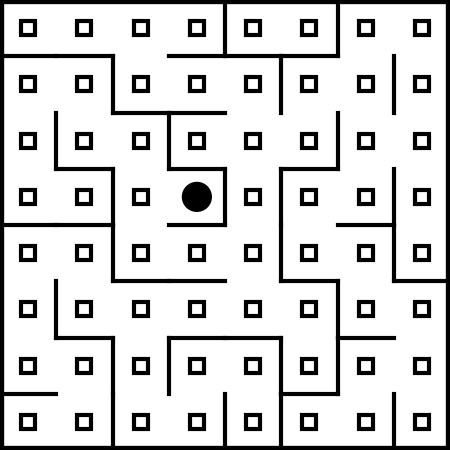
\includegraphics[width=2in]{AE} & 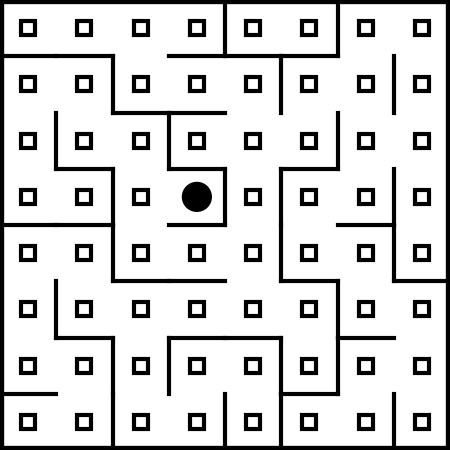
\includegraphics[width=2in]{AE}

\end{tblr}
\end{center}

To realign the radiation control filter, use the buttons below the grid to plan out a path for the radiation control filter to return to the target state from the starting state. A movement in one direction will be canceled out by a movement immediately following it in the opposite direction; thus, any errors made while planning out the path can be corrected. Once the path has been planned out, click the Submit button to execute the realignment. The highlighted square will follow the designated path. If an incorrect step is encountered, an error message will appear and the filter state will reset, allowing you to attempt the realignment again. Once the filter has been properly realigned, the panel status will change to \status{BB} to indicate that no further actions are necessary.

\subsection*{Life Support System}

\overview

Due to internal malfunctions and equipment damage, the life support configuration files may become corrupted. When this happens, it is necessary for the astronaught to reconfirm the crew settings through the digital control panel.

\instruc

On the panel, there are five letter displays laid out in a row, each surrounded on the top and bottom by buttons that can be used to cycle through the available letters for that display. There may be multiple rounds of settings to be confirmed. For each round, choose letters to spell out one of the words in the table below. Only one word will be possible to spell per round.

\begin{center}
\begin{tblr}{
 hlines, vlines,
 rows = {1cm,m}, columns = {2cm,c}
}
 about & admin & after & again & below\\
 optic & orbit & orion & oxide & right
\end{tblr}
\end{center}

Once you have spelled the word on the letter displays, click the submit button to check whether the correct input was given and move onto the next round. Once all rounds have been completed, the status indicator will show the code \status{BB} to signal that the settings have all successfully been restored and the life support system is in working order.

\end{document}
